\documentclass[11pt]{article}

%\usepackage[nosol]{optional}
\usepackage[sol]{optional}

\usepackage {tikz}
    \usetikzlibrary{calc,shapes,arrows,automata,positioning,cd}
    \tikzset{
     dot node/.style={font=\sffamily\small},
      cfgedge/.style   = {black, ->, >=stealth},
      forward/.style = { blue, ->, >=angle 45},
      backward/.style = { red, densely dashed, ->, >=latex' },
      backwardleft/.style = { red, densely dashed, <-, >=latex' },
      position/.style args={#1:#2 from #3}{
        at=(#3.#1), anchor=#1+180, shift=(#1:#2)
    },
    }
    \usepackage{xcolor}

\usepackage{listings, ../listings-rust/listings-rust}
\usepackage{listings}
\usepackage{xcolor}
\definecolor{codegreen}{rgb}{0,0.6,0}
\definecolor{codegray}{rgb}{0.5,0.5,0.5}
\definecolor{codepurple}{rgb}{0.58,0,0.82}
\definecolor{backcolour}{rgb}{0.95,0.95,0.92}
\lstset{
    language=Python,
    keepspaces=true,
    numbers=left,
    backgroundcolor=\color{backcolour},
    commentstyle=\color{codegreen},
    basicstyle=\ttfamily,
    otherkeywords={self,True,False,yield},
    keywordstyle=\ttfamily\color{blue!90!black},
    %basicstyle=\footnotesize,
    keywords=[3]{ttk},
    keywordstyle={[2]\ttfamily\color{orange!80!orange}},
    keywordstyle={[3]\ttfamily\color{red!80!orange}},
    emph={MyClass,__init__},
    emphstyle=\ttfamily\color{red!80!black},
    stringstyle=\color{green!80!black},
    showstringspaces=false
}

\newcommand{\N}{\mathbb{N}}
\newcommand{\Z}{\mathbb{Z}}

% For proof.
\usepackage{amsmath,amsthm,amssymb}

\usepackage{enumerate}
\usepackage{graphicx}
\usepackage{float}
\usepackage{subcaption}
\usepackage{comment}

\renewcommand{\topfraction}{.9}
\renewcommand{\textfraction}{.1}

\usepackage{fullpage,amsmath,amssymb}
\usepackage[colorlinks=true,citecolor=blue,linkcolor=blue]{hyperref} % for href links, and also makes \ref and \eqref clickable in the PDF

% parenthetical comment to state verbally but not write on the board
\newcommand{\com}[1]{\footnote{#1}}

\newcommand{\deltahat}{\widehat{\delta}}

\newcommand{\QuasiP}{\mathsf{QuasiP}}

\newcommand{\TIME}{\mathsf{TIME}}

\usepackage{fancyhdr}
\fancypagestyle{firststyle}
{
    \fancyhf{}
    \fancyhead[C]{Copyright \copyright\ \today, David Doty}
}


\title{Homework 5 \opt{sol}{Solutions} -- ECS 220, Winter 2020}
\date{}
\newtheorem{theorem}{Theorem}
\begin{document}
\maketitle
\thispagestyle{firststyle}
\vspace{-2.0cm}

\section{$2\textsc{Sat}$ is to $\mathsf{NL}$ as $3\textsc{Sat}$ is to $\mathsf{NP}$. (Textbook problem 8.8)}
\begin{quote}
    Show that $2\textsc{Sat}$ is $\mathsf{NL}$-complete.
    {\bf Hint:} first use the discussion in Section 4.2.2 to reduce
    $\textsc{Reachability}$ to the problem $2\textsc{UnSat}$,
    the problem of whether a $2\textsc{Sat}$ formula is unsatisfiable,
    and then use the Immerman-Szelepcs\'{e}nyi Theorem.
    %Can you invent a restricted case of $2\textsc{Sat}$ that is $\mathsf{L}$-complete?
\end{quote}

\section*{Solution}

\subsection*{Proof idea}

Thanks to Immerman-Szelepcs\'{e}nyi Theorem, to prove $2\textsc{Sat}$ is $\mathsf{NL}$-complete, we only need to prove $2\textsc{UnSat}$ is $\mathsf{NL}$-complete.
Therefore, the whole prove will be focused in $2\textsc{UnSat}$ is $\mathsf{NL}$-complete.

We would be using the fact that if there is a loop in the implication graph, the corresponding formula would be unsatisfiable.
Therefore the general idea for reduction is to take any \textit{acyclic} graph $G_a$, consider each directed edge($x \rightarrow y$) to be a clause($\bar{x} \vee y$).
Then we create an edge(add a clause) $t \rightarrow s$($\bar{t} \vee s$), if there is a path from $s$ to $t$, this would make it a loop and thus unsatisfiable.
This is how we solve $\textsc{Reachability}$ using $2\textsc{UnSat}$.

There is one last piece in that reduction, the graph has to be \textit{acyclic}, but $\textsc{Reachability}$ talks about any graph.
This issue is important because if the graph contains a loop itself, the reduced formula would be automatically unsatisfiable, regardless if there is a path from $s$ to $t$.
We were stuck at this for a long time, until we found that \href{https://people.cs.umass.edu/~barring/cs601sum03/hw/4sol.html}{this proof} that $\textsc{Reachability} \le_L \textsc{AcyclicReachability}$ and thus $\textsc{Acyclic-Reachability} \in \mathsf{NL}-complete$.

To sum up, we would be proving $2\textsc{UnSat}$ is $\mathsf{NL}$ real quick.
Then we would sketch a quick proof that $\textsc{Reachability} \le_L \textsc{AcyclicReachability}$, our reduction will show that $\textsc{AcyclicReachability} \le_L 2\textsc{UnSat}$.
Therefore we have $\textsc{Reachability} \le_L 2\textsc{UnSat}$.
Since $\textsc{Reachability}$ is $\mathsf{NL}$-complete, so do $2\textsc{UnSat}$, using Immerman-Szelepcs\'{e}nyi Theorem,  $2\textsc{Sat}$ is $\mathsf{NL}$-complete

\subsection*{$\mathsf{NL}$}

\begin{theorem}
    $2\textsc{UnSat}$ is $\mathsf{NL}$.
\end{theorem}
\begin{proof}
    Thanks to the discussion in Section 4.2.2, we have a log space reduction to reduce $2\textsc{UnSat}$ to a graph $G_a$.
    (Quick recall: $a \vee b$ become 4 vertices $a, b, \bar{a}, \bar{b}$ and 2 edges $\bar{a} \rightarrow b, \bar{b} \rightarrow a$).

    From the duscission we know that if $\exists x, \bar{x}$ that are connected in $G_a$, $2\textsc{UnSat}$ returns true as the variable corresponding to $x$ cannot be set.
    Therefore, we can use $\textsc{Reachability}$ to help solve $2\textsc{UnSat}$.

    \begin{lstlisting}[language = Rust]
fn two_un_sat(Clause: clause) -> bool{
    let graph = Graph::new(clause);
    for vertex in graph.vertices{
        if reachible(&graph, vertex, vertex.bar()) {
            return true;
        }
    }
    false
}\end{lstlisting}

    Now we know in log space reductio ntime can use $\textsc{Reachability}$ to solve $2\textsc{UnSat}$, i.e. $2\textsc{UnSat} \le_L \textsc{Reachability}$

    Since $\textsc{Reachability} \in NL$, $2\textsc{UnSat} \in NL$.
    Using Immerman-Szelepcs\'{e}nyi Theorem, $2\textsc{Sat} \in NL$
\end{proof}

\subsection*{$\textsc{AcyclicReachability} \le_L 2\textsc{UnSat}$}

\subsubsection*{Reduction}

$\forall$ acyclic graph $G_a$, consider each of its edge a an implication, i.e. edge $x \rightarrow y$ is reduced to $\bar{x} \vee y$.
Finally we would add clause $()\bar{t} \vee s) \wedge (t \vee s) \wedge (\bar{t} \vee \bar{s})$, which corresponds to edge $t \rightarrow s$, connect all clauses and we call it $\phi_G$.

Also, let denote $G_a'$ as the implication graph of $\phi_G$, since we have $\bar{t} \vee s$, edge $t \rightarrow s$ is in $G$.

\subsubsection*{Example}

The following graph shows an example of how to do the reduction.

\begin{figure}[h]
    \centering
    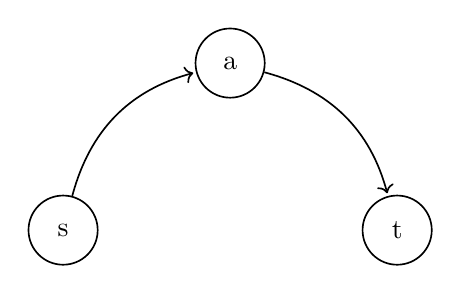
\begin{tikzpicture}[shorten >=1pt,node distance=3cm,on grid,auto, semithick]
        \node [state] (a)                       {a};
        \node [state] (b) [below left of=a]     {s};
        \node [state] (c) [below right of=a]    {t};

        \path[->]
        (b) edge [bend left] node  {} (a)
        (a) edge [bend left] node  {} (c);
    \end{tikzpicture}
    \caption{$G_a$: Original graph}
\end{figure}

And this $G_a$ gets the following $\phi_G$:

$$ (\bar{s} \vee a) \wedge (\bar{a} \vee t) \wedge (\bar{t} \vee s) \wedge (t \vee s) \wedge (\bar{t} \vee \bar{s})$$

\begin{figure}[h]
    \centering
    \begin{tikzpicture}[shorten >=1pt,node distance=3cm,on grid,auto, semithick]
        \node [state] (a)                       {a};
        \node [state] (b) [below left of=a]     {s};
        \node [state] (ns) [right of=c]     {$\bar{s}$};
        \node [state] (c) [below right of=a]    {t};
        \node [state] (nt) [left of=b]     {$\bar{t}$};

        \path[->]
        (b) edge [bend left] node  {} (a)
        (a) edge [bend left] node  {} (c)
        (c) edge [bend left] node  {} (b)
        (c) edge [bend left] node  {} (ns)
        (nt) edge [bend left] node  {} (b);
    \end{tikzpicture}
    \caption{$G_a'$: Implication graph of $\phi_G$}
\end{figure}


\subsubsection*{Space complexity}

Since we do all the change on the fly, i.e. we know what to do by simply look at each edge, the space complexity is O(1).

\subsubsection*{Proof it works}

\begin{theorem}
    Acyclic graph $G_a$ has path from $s$ to $t$ iff $\phi_G$ is unsatisfiable.
\end{theorem}
\begin{proof}
    $\Rightarrow$ If $G_a$ has a path from $s$ to $t$, we woul nonate it as:

    $$s \rightarrow c_1 \rightarrow \cdots \rightarrow c_k \rightarrow t$$

    Such path would be converted to:

    $$(\bar{s} \vee c_1) \wedge (\bar{c_1} \vee c_2) \wedge \cdots \wedge (\bar{c_{k-1}} \vee c_k) \wedge (\bar{c_k} \vee t) \wedge (t \vee s) \wedge (\bar{t} \vee \bar{s})$$

    Since we also added $\bar{t} \vee s$, it's clear that $\phi_G$ must have all the variables set to true or false.
    But $s$ and $t$ cannot be the same, since $(t \vee s) \wedge (\bar{t} \vee \bar{s})$

    $\Leftarrow$

    Since $\phi_G$ is not satisfiable, then the implication graph $G_a'$ must has a loop.
    But $G_a$ is acyclic graph and $G_a'$ and $G_a$ only differs in one edge.

    Therefore it is safe to conclude that the loop must be introduced by that extra edge $t \rightarrow s$.
    And thus we know there must be an edge from $s$ to $t$.
\end{proof}

\subsection*{$\textsc{Reachability} \le_L \textsc{AcyclicReachability}$}

\subsubsection*{Reduction}

To take apart possible circles we would take a 2D graph to 3D.
From any directed graph $G = (V, E)$ let's construct an acyclic graph $G_a = (V_a, E_a)$.

$G_a$ consists of $|V|$ layers, the intuition is that the max length from $s$ to $t$ would be $|V| - 1$.
To put it formally, we have:
$$V = V_1 = V_2 = \cdots = V_{|V|}$$
$$V_a = V_1 \cup V_2 \cup \cdots \cup V_{|V|}$$

$V_k$ represent the k-th layer of $G_a$, and we would use $x_k$ to notate vertex $x \in V$ in the k-th layer.

Edge are consists of two parts: original edges, which is now altered to set between layers, and the added edges.

$$E_{alt} = \{(x_i, y_{i+1}) | \forall 1 \le i \le |V| - 1, \forall (x, y \in E)\}$$
$$E_{add} = \{(t_i, t_{i+1}) | \forall 1 \le i \le |V| - 1\}$$

We add edges between $t_i$ and $t_{i+1}$ so that we can arrive at an early layer and directly jump to the end.

Now, the quest is converted from "find a path between $s$ and $t$" to "find a path from $s_1$ to $t_{|V|}$" and we shall prove that the two job are actually the same.
But before we do that, let's see some example to make sure we are clear about the reduction.

\subsubsection*{Example}
\begin{figure}[h]
    \centering
    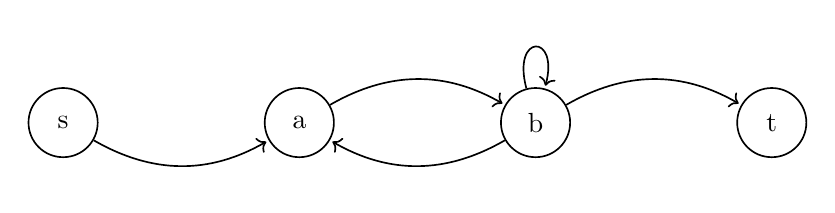
\begin{tikzpicture}[shorten >=1pt,node distance=3cm,on grid,auto, semithick]
        \node [state] (s)                  {s};
        \node [state] (a) [right of=s]    {a};
        \node [state] (b) [right of=a]    {b};
        \node [state] (t) [right of=b]    {t};

        \path[->]
        (s) edge [bend right] node  {} (a)
        (a) edge [bend left] node  {} (b)
        (b) edge [bend left] node  {} (t)
        (b) edge [bend left] node  {} (a)
        (b) edge [loop above] node  {} ();
    \end{tikzpicture}
    \caption{$G$: Original graph}
\end{figure}

\begin{figure}[h]
    \centering
    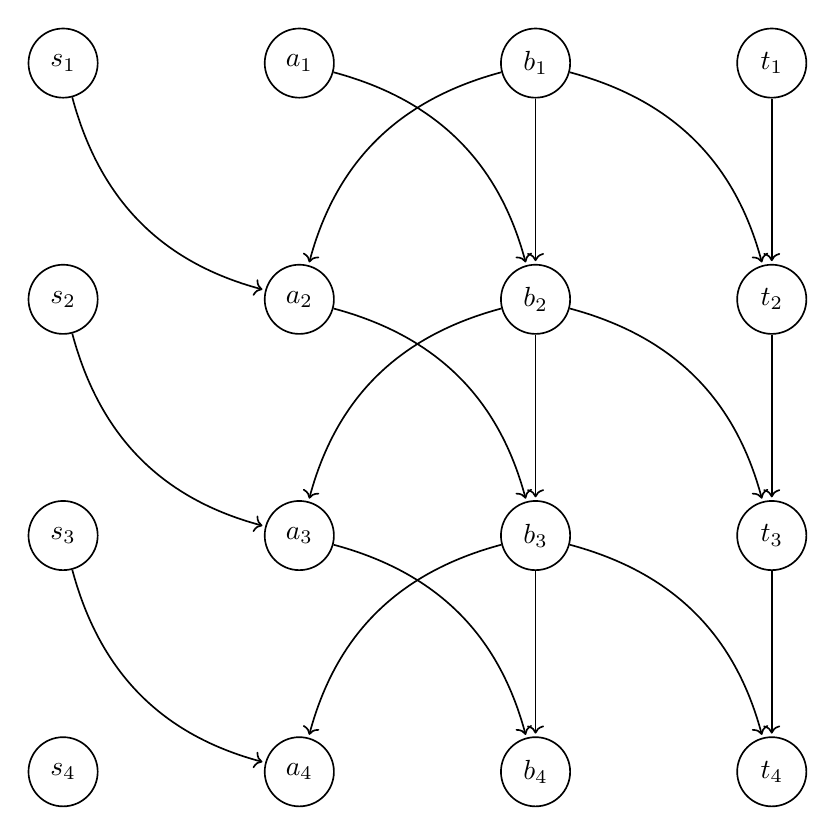
\begin{tikzpicture}[shorten >=1pt,node distance=3cm,on grid,auto, semithick]
        \node [state] (s1)                  {$s_1$};
        \node [state] (a1) [right of=s1]    {$a_1$};
        \node [state] (b1) [right of=a1]    {$b_1$};
        \node [state] (t1) [right of=b1]    {$t_1$};

        \node [state] (s2) [below of=s1]    {$s_2$};
        \node [state] (a2) [right of=s2]    {$a_2$};
        \node [state] (b2) [right of=a2]    {$b_2$};
        \node [state] (t2) [right of=b2]    {$t_2$};

        \node [state] (s3) [below of=s2]    {$s_3$};
        \node [state] (a3) [right of=s3]    {$a_3$};
        \node [state] (b3) [right of=a3]    {$b_3$};
        \node [state] (t3) [right of=b3]    {$t_3$};

        \node [state] (s4) [below of=s3]    {$s_4$};
        \node [state] (a4) [right of=s4]    {$a_4$};
        \node [state] (b4) [right of=a4]    {$b_4$};
        \node [state] (t4) [right of=b4]    {$t_4$};
        \path[->]
        (s1) edge [bend right] node  {} (a2)
        (s2) edge [bend right] node  {} (a3)
        (s3) edge [bend right] node  {} (a4)

        (a1) edge [bend left] node  {} (b2)
        (a2) edge [bend left] node  {} (b3)
        (a3) edge [bend left] node  {} (b4)

        (b1) edge [bend left] node  {} (t2)
        (b2) edge [bend left] node  {} (t3)
        (b3) edge [bend left] node  {} (t4)

        (b1) edge [bend right] node  {} (a2)
        (b2) edge [bend right] node  {} (a3)
        (b3) edge [bend right] node  {} (a4)

        (b1) edge  node  {} (b2)
        (b2) edge  node  {} (b3)
        (b3) edge  node  {} (b4)

        (t1) edge  node  {} (t2)
        (t2) edge  node  {} (t3)
        (t3) edge  node  {} (t4);
    \end{tikzpicture}
    \caption{$G_a$: 4-layer graph generated from $G$, the task would be to find a path from $s_1$ to $t_4$}
\end{figure}

\subsubsection*{Proof that the reduction generates acyclic graph}

\begin{theorem}
    The graph $G_a$ generated is acyclic
\end{theorem}
\begin{proof}
    This is trivial since there is no edge connecting node in the same layer nor the upper later, the edge always goes down.
    There can't be loops.
\end{proof}

\subsubsection*{Space Complexity}

Again  the process requires no memory to record anything, thus the space complexity is O(1).

\subsubsection*{Proof that the reduction works}

\begin{theorem}
    There is a path from $s$ to $t$ in $G$ iff there is a path from $s_1$ to $t_|V|$ in $G_a$.
\end{theorem}

\begin{proof}
    $\Rightarrow$ If there is a path $s \rightarrow a^2 \rightarrow a^3 \rightarrow \cdots \rightarrow a^{k-1} \rightarrow t$.
    (Let's annotate $s$ as $a^1$ and $t$ as $a^k$)

    It is safe to assume the following: there is no loop in this path, as it would then be possible to find a shorter path from $s$ to $t$.
    Thus if must follows that $k \le |V| - 1$.

    The path in $G_a$ would be $$s_1 \rightarrow a^2_2 \rightarrow a^3_3 \rightarrow \cdots \rightarrow a^{k-1}_{k-1} \rightarrow t_k \rightarrow t_{k+1} \rightarrow \cdots \rightarrow t_{|V|}$$

    $\Leftarrow$
    The left side is similar, if there is a path in $G_a$, we can convert it back, using the layer as the number of steps.
\end{proof}

Therefore, we have concluded that $\textsc{Reachability} \le_L \textsc{AcyclicReachability}$.

\subsection*{Conclusion}

We have proved that $\textsc{Reachability} \le_L \textsc{AcyclicReachability} \le_L 2\textsc{UnSat}$.
Since we also know that $2\textsc{UnSat}$ is $\mathsf{NL}$, we can conclude that $2\textsc{UnSat}$ is $\mathsf{NL}$-complete.
Using  Immerman-Szelepcs\'{e}nyi Theorem, we know  $2\textsc{Sat}$ is $\mathsf{NL}$-complete too.

Along the way we referred \href{https://people.cs.umass.edu/~barring/cs601sum03/hw/4sol.html}{this proof} to provide inspiration of how to prove $\textsc{Reachability} \le_L \textsc{AcyclicReachability}$ and thus $\textsc{Acyclic-Reachability} \in \mathsf{NL}-complete$.
\end{document}